% CS F407 Artificial Intelligence: final project report template.
% Limit: 2 pages, including everything except references.
% Do not change the font size, margins or spacing.
\documentclass[11pt,a4paper,twocolumn]{article}

\usepackage[margin=2cm,columnsep=0.8cm]{geometry}
\usepackage[T1]{fontenc}
\usepackage{lmodern}
\usepackage{microtype}
\usepackage{amsmath,amssymb}
\usepackage{graphicx}
\usepackage{booktabs}
\usepackage{tabularx}
\usepackage{enumitem}
\usepackage{titlesec}
\usepackage[hidelinks]{hyperref}

\titleformat{\section}{\normalsize\bfseries}{\thesection}{0.6em}{}
\titlespacing*{\section}{0pt}{1.2ex plus 0.3ex}{0.6ex}
\setlist{nosep,leftmargin=*}
\setlength{\parskip}{0.3ex}

\newcommand{\coursename}{CS F407 Artificial Intelligence, AY 2026--27 Semester I}
\newcommand{\teamno}{Team LogicForge}
\newcommand{\githuburl}{https://github.com/f20241463-cmd/CS-F407-chaturanga}

\begin{document}

\twocolumn[{%
\begin{center}
  {\large\bfseries ChaturangZero: Learning Chaturanga from Self-Play Alone}\\[1ex]
  \teamno\\
  Nandika Tamse (2024A1PS1463G), Avisha Srivastava (2024A1PS0273G), Srinivasa Harshith Pataneni (2024A7PS0597G)\\[0.5ex]
  {\small \coursename, BITS Pilani, K.K. Birla Goa Campus}\\[1.5ex]
  \begin{minipage}{0.85\textwidth}
    \small
    \centerline{\bfseries Abstract}\vspace{0.5ex}
    We built ChaturangZero, an AlphaZero-style agent for Chaturanga, the ancient Indian
    ancestor of chess, that is given only the rules. A small residual network guides Monte
    Carlo Tree Search, and the network learns from games the agent plays against itself.
    Under the course limits (50 simulations per move, at most 6 blocks of 128 filters) and on
    one laptop, plain AlphaZero training stalled after 54,000 games: about 85\% of self-play
    games were drawn, so the value head had little to learn from. Switching to Gumbel
    self-play, which trains on an improved policy instead of visit counts, kept improving for
    another 78,000 games. The final model beats our first strong model 91 wins to 4 at 1600
    simulations, beats a greedy-capture player 80 to 3, and is about 300 rating points
    stronger. An experienced human (FIDE blitz 1641) still beats it, which matches our
    estimate that mastery needs hundreds of times more games.
  \end{minipage}
\end{center}
\vspace{1.5ex}
}]

\section{Introduction}
AlphaZero~\cite{silver2018alphazero} showed that one algorithm can learn chess, shogi and Go
to superhuman level from the rules alone, by combining tree search with a neural network
trained on self-play. Our goal was to build that method from scratch for Chaturanga and to
measure how far it gets on the compute of a course project. The input to our system is a
position; the output is a move and an estimate of who is winning.

The course proposal fixed the constraints: no human knowledge beyond the rules (no opening
books, piece values or hand-written evaluation), 30 to 50 MCTS simulations per move in
training, a residual network of 4 to 6 blocks with 64 to 128 filters, and a 4096-wide
action space. It also set four milestones: a rules engine verified by unit tests, MCTS
working with an untrained network, a self-play pipeline, and benchmarks against earlier
iterations and baseline players with learning curves. All four are complete.

Our contributions are: (1) a tested rules engine and a full AlphaZero pipeline that runs on
one laptop; (2) a measured account of why plain AlphaZero stalls on this game at our scale,
including over a dozen changes that did not help; and (3) Gumbel self-play, which removed the
stall and gave a final model about 300 Elo above our first strong model.

\section{Background and related work}
Game playing by search is a core AI topic~\cite{russell2021aima}. Monte Carlo Tree Search
grows a game tree by sampling, balancing promising and untried moves with bandit
rules~\cite{kocsis2006bandit}; PUCT adds a prior over moves to that
rule~\cite{rosin2011puct}. AlphaGo Zero and AlphaZero~\cite{silver2017go,silver2018alphazero}
combine PUCT search with a residual network~\cite{he2016resnet} that predicts a move
distribution and a game result, and train it only from self-play, with 800 simulations per
move and millions of games. Gumbel AlphaZero~\cite{danihelka2022gumbel} replaces root noise
and visit-count targets with sampling without replacement, sequential halving and an
improved policy, and is designed to work with very few simulations, which is the regime the
course limits put us in. We also tried ideas from KataGo~\cite{wu2019katago} (a moves-left
head) and MuZero~\cite{schrittwieser2020muzero} (Reanalyse).

\textbf{The game.} Chaturanga is played on an uncheckered $8\times8$
board~\cite{murray1913history}. Pieces stand as in chess, with the Raja (king) on the
d-file and the Mantri (counselor) on the e-file:

\begin{table}[h]
\centering
\small
\begin{tabular}{@{}ll@{}}
\toprule
Piece & Move \\
\midrule
Raja (king) & one square in any direction \\
Mantri (counselor) & one square diagonally \\
Ratha (chariot) & any distance orthogonally \\
Gaja (elephant) & two squares diagonally (jumps) \\
Ashva (horse) & as a chess knight \\
Padati (soldier) & one forward, captures \\
 & diagonally, promotes to Mantri \\
\bottomrule
\end{tabular}
\caption{Pieces. No castling, double step or en passant.}
\label{tab:pieces}
\end{table}

\noindent Checkmate wins. Stalemate, threefold repetition and 100 plies without a capture
or pawn move are draws. Because the Mantri and Gaja are short-range, an advantage is much
harder to turn into checkmate than in chess, and this shapes everything below.

\section{Method}
\textbf{Encoding.} A position is 13 planes of $8\times8$: one per piece type and color, plus
the side to move. A move is $\text{from}\cdot64+\text{to}$, giving 4096 actions, and
illegal actions are masked out before the softmax.

\textbf{Network.} An input $3\times3$ convolution to 64 filters, 4 residual blocks (two
$3\times3$ convolutions with batch normalization and a skip connection), a policy head
($1\times1$ convolution, then a linear layer to 4096 logits) and a value head ($1\times1$
convolution, a 64-unit layer, $\tanh$), 836k parameters in all. For a position with target
policy $\pi$ and final result $z\in\{-1,0,1\}$ for the side to move, the loss is
\begin{equation}
\ell = (z - v)^2 - \pi^\top \log p + c\,\lVert\theta\rVert^2,\quad c=10^{-4}.
\end{equation}

\textbf{Search.} Each simulation descends the tree by picking the child that maximizes
\begin{equation}
-Q(s') + c_{\text{puct}}\, P(s,a)\,\frac{\sqrt{N(s)}}{1+N(s')},\quad c_{\text{puct}}=1.5,
\end{equation}
where $Q(s')$ is the child's mean value from the child's side, $P$ the network prior and $N$
visit counts. A new leaf is expanded with the network's priors, and its value is backed up
with the sign flipped each ply. There are no random rollouts. In plain self-play, Dirichlet
noise ($\alpha=0.3$, weight 0.25) is mixed into the root priors and moves are sampled in
proportion to visit counts, which are also the policy target.

\textbf{Self-play and training.} Each iteration plays 100 games at 50 simulations per move,
adds every position to a replay buffer of the latest 250,000, and takes 500 Adam steps of
batch 256. Games stop at 800 plies and count as draws. One rules-only addition: the agent
never picks a move that causes threefold repetition unless every searched move does.

\textbf{Gumbel self-play.} At the root we add Gumbel noise $g$ to the logits, keep the top
$k$ moves, and split the 50 simulations among them by sequential halving (each round, the
better half by $g + \text{logits} + \sigma(\hat q)$ survives). The policy target is the
improved policy
\begin{equation}
\pi' = \text{softmax}\big(\text{logits} + \sigma(\hat q)\big),
\end{equation}
with $\sigma(\hat q) = (50 + \max N)\, c_{\text{scale}}\, \hat q$, where $\hat q$ is the searched value of each move, or the network's value for unsearched
ones. Every legal move gets credit, not only the few that 50 visits reach. Below the root,
and in every evaluation match and human game, the PUCT search is unchanged.

\textbf{Implementation.} Plain Python with NumPy and PyTorch. 166 unit tests cover the rules
(check, mate, stalemate, promotion and every draw rule), the search (including a toy game
with a known best move), value-target signs, policy targets, a full small training run and
the evaluation tools. We made self-play about 11 times faster without changing its output
(259 to 19\,ms per move: cached legal moves, precomputed move tables, batch normalization
folded into convolutions), then batched the network calls of many games onto the laptop's
GPU, which halved self-play time again. A test checks the fast engine against the original
on 3,000 random positions.

\section{Experimental setup}
\textbf{Training.} Table~\ref{tab:stages} lists the stages. Each Gumbel stage was checked
in 200-game matches against the previous model; for the last one we fixed in advance
that a new final model must score at least 0.55 against the old one.

\begin{table}[h]
\centering
\small
\begin{tabular}{@{}llrr@{}}
\toprule
Iterations & Self-play & Games & Hours \\
\midrule
1--560 & plain PUCT & 54k & 151 \\
560--1220 & Gumbel $k{=}16$ & 66k & 39 \\
1220--1280 & Gumbel $k{=}32$ & 6k & 3.3 \\
1280--1340 & $k{=}32$, $c_{\text{scale}}{=}0.03$ & 6k & 3.8 \\
\bottomrule
\end{tabular}
\caption{Training stages ($c_{\text{scale}}=0.1$ unless stated). Learning rate $10^{-3}$
lowered to $3\times10^{-5}$ for plain training, $10^{-4}$ to $3\times10^{-5}$ for Gumbel. In total about 132,000
games and 200 hours on one laptop (6 CPU cores, Apple GPU).}
\label{tab:stages}
\end{table}

\textbf{Evaluation.} Head-to-head matches of 100 to 400 games at 50 simulations,
temperature 0.3, no root noise, repetition avoidance, alternating colors and an 800-ply
cap. The score is $(\text{wins}+\tfrac12\text{draws})/\text{games}$ with a 95\% margin of
$1.96\sqrt{p(1-p)/n}$. Baselines: random moves, a greedy player that captures the most
valuable piece it can (its piece values are used only by this baseline, never by our
agent), and the same MCTS with an untrained network. To put all models on one scale we fit
maximum-likelihood Elo ratings to all 141 matches (24,217 games), draws as half a win, with
iteration 560 fixed at 0 and 90\% ranges from 100 resamples. Humans played the agent in a
browser at 800 simulations per move.

\section{Results}
\textbf{Learning curve.} Figure~\ref{fig:curve} shows the Elo of saved models. Plain training
beat its random start 27--0 and reached iteration 560, which beat random and untrained play
but drew 99 of 100 games against greedy capture and rarely gave checkmate. A lower learning
rate gave its last clear gain; after that, every continuation stayed level. Gumbel self-play
was the largest step: 1220 beats 560 by 83 wins to 1 at 1600 simulations (0.927) and 0.814
at 50 simulations, and decisive self-play games rose from about 15\% to 44\%. Then $k=32$
(1280: 0.580 against 1220) and $c_{\text{scale}}=0.03$ (1340: 0.553 against 1280 over 400
games) each added a smaller step.

\begin{figure}[t]
\centering
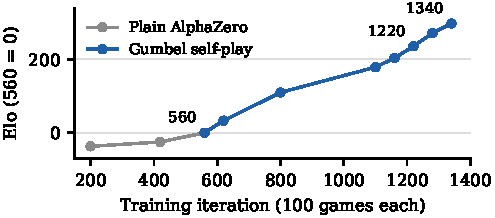
\includegraphics[width=\linewidth]{learning_curve.pdf}
\caption{Learning curve: Elo of saved models against training iteration (560 at 0, 90\%
ranges about $\pm$20).}
\label{fig:curve}
\end{figure}

\textbf{Against fixed opponents.} Table~\ref{tab:bench} compares 560 and the final model.
The final model wins most games, mostly by checkmate (18 of 30 against random, 21 of 30
against greedy capture, against 3 and 1 for 560).

\begin{table}[h]
\centering
\small
\begin{tabular}{@{}lcc@{}}
\toprule
Opponent (100 games) & Iter.\ 560 & Final (1340) \\
\midrule
Random moves & 16--0, 0.58 & 59--0, 0.80 \\
Untrained + MCTS & 17--4, 0.57 & 66--0, 0.83 \\
Greedy capture & 0--1, 0.50 & 80--3, 0.89 \\
560, both at 1600 sims & -- & 91--4, 0.94 \\
\bottomrule
\end{tabular}
\caption{Wins--losses (draws make up the rest) and score. Higher is better.}
\label{tab:bench}
\end{table}

\textbf{What did not help.} Table~\ref{tab:neg} lists changes that each continued a model
for 60 to 140 iterations and then played it. None beat its starting point outside the
margin. A $6\times128$ network trained from scratch with the same recipe and games as a
$4\times64$ one lost slightly to it (0.459), so network size was not the limit.

\begin{table}[h]
\centering
\small
\begin{tabular}{@{}lc@{}}
\toprule
Change (from 560 unless stated) & Score \\
\midrule
Learning rate $2\times10^{-5}$, 140 iterations & 0.515 \\
Draws valued $-0.2$ instead of 0 & 0.454 \\
Search values mixed into value targets & 0.518 \\
Self-play games capped at 300 plies & 0.500 \\
Averaged weights of 7 checkpoints & 0.515 \\
More root noise / late starts & 0.47 / 0.50 \\
Decisive games weighted 3 / mirror & 0.50 / 0.51 \\
Older opponents in self-play & 0.497 \\
Moves-left head / Reanalyse & 0.48 / 0.48 \\
$6\times128$ net (trained on 560's games) & 0.495 \\
From 1220: 1000 training steps & 0.41 \\
From 1220: buffer 100k / lr $3{\cdot}10^{-4}$ & 0.43 / 0.32 \\
\bottomrule
\end{tabular}
\caption{Score of each change against its starting model (100 to 200 games, margin
about $\pm$0.03 to 0.05; 0.5 is even).}
\label{tab:neg}
\end{table}

\textbf{More search at play time.} The simulation limit applies to training only.
Against itself at 50 simulations, the model at 800 scored 23--0 (0.616); 1600 beat 800
15--3 (0.560), and 3200 was no better than 1600 (0.505). The browser game uses 1600, about
half a second per move.

\textbf{Against people.} A team member new to chess beat an early model (6 games, 3 wins
and 3 draws). An experienced player (FIDE blitz 1641) then played later models
(Table~\ref{tab:human}).

\begin{table}[h]
\centering
\small
\begin{tabular}{@{}lcc@{}}
\toprule
Model & Human W--D--L & Agent score \\
\midrule
Iteration 560 & 5--3--2 & 0.35 \\
Iteration 1220 & 13--2--0 & 0.07 \\
Iteration 1280 & 12--1--0 & 0.04 \\
Final (1340) & 11--1--0 & 0.04 \\
\bottomrule
\end{tabular}
\caption{FIDE 1641 player against the agent at 800 simulations.}
\label{tab:human}
\end{table}

\noindent Being stronger against programs did not make the agent harder for this player,
who had also learned its style: the human wins by collecting material the agent gives away
in quiet positions, then mating, usually in under 120 plies.

\section{Discussion and limitations}
\textbf{Why plain training stalls.} With about 85\% of self-play games drawn, nearly every
value target is 0, so the value head learns little; in our first run, 81\% of its
predictions were within 0.05 of 0. A resignation test showed the same thing: of 34 games
in which the agent would have resigned at a value of $-0.3$, 32 were not lost. The value
head does not see a loss coming, and decisive games come from sudden blunders rather than
built-up advantages. Pushing for more decisive games did not fix this: shorter games
gave more of them but no gain, and a draw penalty made play weaker.

\textbf{Why Gumbel helped.} At 50 simulations, visit counts are a coarse target: a good move
the search never visits gets no credit. The improved policy gives every legal move a
target from its prior and, where searched, its value. With the same network, simulations and
loss, this kept improving for 660 iterations where every other continuation stalled, and
the extra decisive games gave the value head more real results.

\textbf{Limitations.} The main limit is scale (Table~\ref{tab:scale}). At our speed, 44
million games would take about seven years of nonstop running on this laptop. Chaturanga's
weaker pieces may make it simpler than chess, but it likely still needs millions of games.
Most match games are drawn, so a score says little about how often the agent can win, and
the margins cannot resolve differences below about 0.03. The human sample is small (56 games,
two players).

\begin{table}[h]
\centering
\small
\begin{tabular}{@{}lll@{}}
\toprule
 & AlphaZero & Ours \\
\midrule
Self-play games & 44 million & 132,000 \\
Training sims & 800 & 50 \\
Network & $20\times256$ & $4\times64$ \\
Hardware & 5,000 TPUs & one laptop \\
\bottomrule
\end{tabular}
\caption{Scale compared with AlphaZero: about 330 times fewer games.}
\label{tab:scale}
\end{table}

\textbf{Future work.} Far more games with the larger network, starting from the final
model's games, on several machines; and a value signal that reaches the value head more
often within the rules.

\section{Conclusion}
A full AlphaZero pipeline learns Chaturanga from the rules alone, but at course-sized
compute plain training stalls on drawn games. Gumbel self-play broke that stall and gave a
model about 300 Elo above our first strong one, which beats every baseline mostly by
checkmate. Mastering the game would need hundreds of times more games than one laptop can
play.

\section*{Individual member contributions}
{\small
\begin{tabularx}{\linewidth}{@{}>{\raggedright\arraybackslash}p{3.1cm} >{\raggedright\arraybackslash}X@{}}
\toprule
Name & Contribution \\
\midrule
Nandika Tamse & Rules engine, tensor encoding, move generation, unit tests. \\
Srinivasa Harshith Pataneni & ResNet model and loss, training loop, replay buffer. \\
Avisha Srivastava & MCTS (PUCT, Gumbel), evaluation suite, plots, experiments, report. \\
\bottomrule
\end{tabularx}}

\smallskip
\noindent All members have read this report and agree with the statement above.

\section*{Generative AI disclosure}
We used Claude Code with Claude Opus 5.5 (Anthropic) to write and debug code and experiment
scripts, analyze results, and draft and edit the report and documentation, affecting all code
and all sections. We checked all such output, ran every experiment ourselves, and take
responsibility for it. No LLM is part of the method.

\section*{Code availability}
\noindent Code and data:\\
\url{\githuburl}\\
The repository is public; its README explains how to reproduce the results.

\begin{thebibliography}{9}
\small
\bibitem{russell2021aima}
S.~Russell and P.~Norvig.
\newblock \emph{Artificial Intelligence: A Modern Approach}, 4th edition.
\newblock Pearson, 2021.
\bibitem{kocsis2006bandit}
L.~Kocsis and C.~Szepesv\'ari.
\newblock Bandit based Monte-Carlo planning.
\newblock In \emph{ECML}, 2006.
\bibitem{rosin2011puct}
C.~D.~Rosin.
\newblock Multi-armed bandits with episode context.
\newblock \emph{Annals of Mathematics and Artificial Intelligence}, 61(3), 2011.
\bibitem{silver2017go}
D.~Silver et al.
\newblock Mastering the game of Go without human knowledge.
\newblock \emph{Nature}, 550:354--359, 2017.
\bibitem{silver2018alphazero}
D.~Silver et al.
\newblock A general reinforcement learning algorithm that masters chess, shogi, and Go
  through self-play.
\newblock \emph{Science}, 362(6419):1140--1144, 2018.
\bibitem{he2016resnet}
K.~He, X.~Zhang, S.~Ren and J.~Sun.
\newblock Deep residual learning for image recognition.
\newblock In \emph{CVPR}, 2016.
\bibitem{danihelka2022gumbel}
I.~Danihelka, A.~Guez, J.~Schrittwieser and D.~Silver.
\newblock Policy improvement by planning with Gumbel.
\newblock In \emph{ICLR}, 2022.
\bibitem{wu2019katago}
D.~J.~Wu.
\newblock Accelerating self-play learning in Go.
\newblock arXiv:1902.10565, 2019.
\bibitem{schrittwieser2020muzero}
J.~Schrittwieser et al.
\newblock Mastering Atari, Go, chess and shogi by planning with a learned model.
\newblock \emph{Nature}, 588:604--609, 2020.
\bibitem{murray1913history}
H.~J.~R.~Murray.
\newblock \emph{A History of Chess}.
\newblock Oxford University Press, 1913.
\end{thebibliography}

\end{document}
